% P05 diagnostic figure reliability_bins|development|M06; allowlisted public aggregate points.
% Each point is an aggregate mean or bin over repeated contexts, not an independent sample.
% data_sha256=7f60e425b5fe235c362c21442c3237e1521aad33df8bebdebfd5854e0cfadd4b
\documentclass[tikz,border=5pt]{standalone}
\ifdefined\pdfinfoomitdate\pdfinfoomitdate=1\fi
\ifdefined\pdfsuppressptexinfo\pdfsuppressptexinfo=-1\fi
\ifdefined\pdftrailerid\pdftrailerid{}\fi
\usepackage{pgfplots}
\usepgfplotslibrary{groupplots}
\pgfplotsset{compat=1.18}
\definecolor{p05Blue}{HTML}{0072B2}
\definecolor{p05Orange}{HTML}{E69F00}
\definecolor{p05Green}{HTML}{009E73}
\definecolor{p05Purple}{HTML}{CC79A7}
\definecolor{p05Red}{HTML}{D55E00}
\definecolor{p05Sky}{HTML}{56B4E9}
\begin{document}
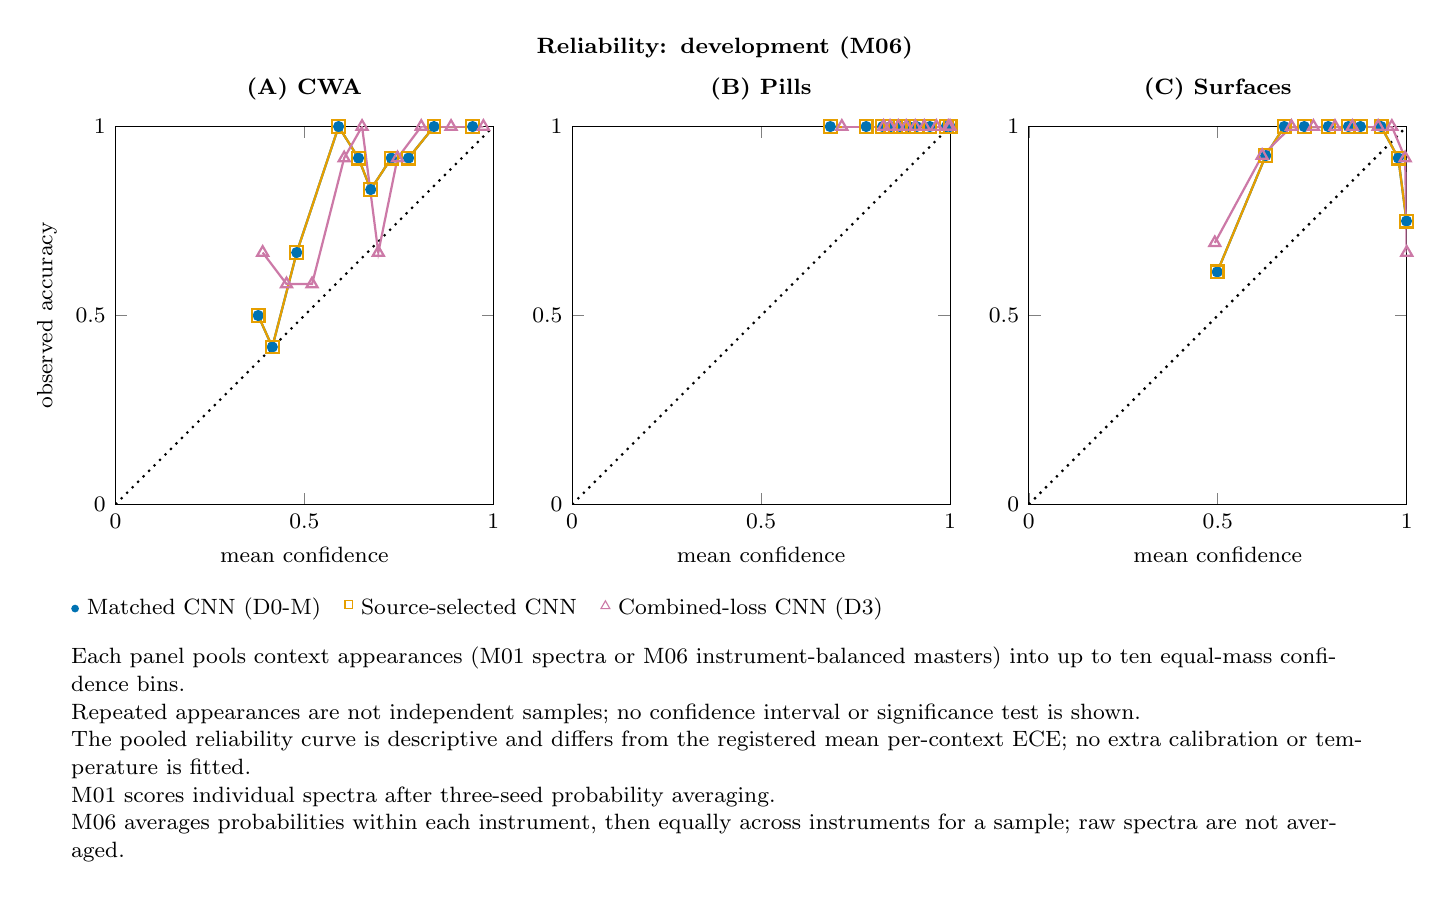
\begin{tikzpicture}
\begin{groupplot}[
  group style={group size=3 by 1, horizontal sep=1.0cm, vertical sep=1.8cm},
  width=4.8cm, height=4.8cm, scale only axis,
  xmin=0, xmax=1, ymin=0, ymax=1,
  xtick={0,0.5,1}, ytick={0,0.5,1},
  tick label style={font=\fontsize{8}{10}\selectfont, color=black},
  label style={font=\fontsize{8}{10}\selectfont, color=black},
  title style={font=\fontsize{8}{10}\selectfont\bfseries, color=black},
]
\nextgroupplot[title={(A) CWA}, xlabel={mean confidence}, ylabel={observed accuracy}]
\addplot[black, dotted, line width=0.8pt] coordinates {(0,0) (1,1)};
\addplot[mark=*, mark size=1.6pt, color=p05Blue, line width=0.8pt, mark options={fill=p05Blue, draw=p05Blue}] coordinates {(0.37782006527168327,0.5) (0.41512694996141736,0.41666666666666669) (0.47972665820623633,0.66666666666666663) (0.59044348697730498,1) (0.64311975957693901,0.91666666666666663) (0.675513740388479,0.83333333333333337) (0.72999671612608363,0.91666666666666663) (0.77563201217080335,0.91666666666666663) (0.84295012278666093,1) (0.94521924104629029,1)};
\addplot[mark=square, mark size=2.3pt, color=p05Orange, line width=0.8pt, mark options={fill=none, draw=p05Orange}] coordinates {(0.37782006527168327,0.5) (0.41512694996141736,0.41666666666666669) (0.47972665820623633,0.66666666666666663) (0.59044348697730498,1) (0.64311975957693901,0.91666666666666663) (0.675513740388479,0.83333333333333337) (0.72999671612608363,0.91666666666666663) (0.77563201217080335,0.91666666666666663) (0.84295012278666093,1) (0.94521924104629029,1)};
\addplot[mark=triangle, mark size=2.3pt, color=p05Purple, line width=0.8pt, mark options={fill=none, draw=p05Purple}] coordinates {(0.38961741125449323,0.66666666666666663) (0.45267693777696422,0.58333333333333337) (0.5203101863145172,0.58333333333333337) (0.60522552983019229,0.91666666666666663) (0.65260017796137937,1) (0.69558630864177029,0.66666666666666663) (0.74638789999769928,0.91666666666666663) (0.80918796156877715,1) (0.88805380359471453,1) (0.97367538308451973,1)};
\nextgroupplot[title={(B) Pills}, xlabel={mean confidence}]
\addplot[black, dotted, line width=0.8pt] coordinates {(0,0) (1,1)};
\addplot[mark=*, mark size=1.6pt, color=p05Blue, line width=0.8pt, mark options={fill=p05Blue, draw=p05Blue}] coordinates {(0.68318206630664791,1) (0.77805239995689512,1) (0.82170870568130849,1) (0.84316116905188798,1) (0.86764324136160798,1) (0.89067672947829257,1) (0.91118574975262212,1) (0.94637575659503814,1) (0.99015052940257464,1) (0.99999999998319145,1)};
\addplot[mark=square, mark size=2.3pt, color=p05Orange, line width=0.8pt, mark options={fill=none, draw=p05Orange}] coordinates {(0.68318206630664791,1) (0.77805239995689512,1) (0.82170870568130849,1) (0.84316116905188798,1) (0.86764324136160798,1) (0.89067672947829257,1) (0.91118574975262212,1) (0.94637575659503814,1) (0.99015052940257464,1) (0.99999999998319145,1)};
\addplot[mark=triangle, mark size=2.3pt, color=p05Purple, line width=0.8pt, mark options={fill=none, draw=p05Purple}] coordinates {(0.71365214826887446,1) (0.82423019378300766,1) (0.84133055177161842,1) (0.86315117348116899,1) (0.88402745275854033,1) (0.90793562329082977,1) (0.93191179692389403,1) (0.96392118525050952,1) (0.99532843717192532,1) (0.99999999999999978,1)};
\nextgroupplot[title={(C) Surfaces}, xlabel={mean confidence}]
\addplot[black, dotted, line width=0.8pt] coordinates {(0,0) (1,1)};
\addplot[mark=*, mark size=1.6pt, color=p05Blue, line width=0.8pt, mark options={fill=p05Blue, draw=p05Blue}] coordinates {(0.49859895668747539,0.61538461538461542) (0.626967973974491,0.92307692307692313) (0.67582863129463933,1) (0.72879711915751078,1) (0.7923615709356292,1) (0.84564178188474548,1) (0.87757571251048627,1) (0.93203423404404095,1) (0.97773775879007252,0.91666666666666663) (0.99934431779483679,0.75)};
\addplot[mark=square, mark size=2.3pt, color=p05Orange, line width=0.8pt, mark options={fill=none, draw=p05Orange}] coordinates {(0.49859895668747539,0.61538461538461542) (0.626967973974491,0.92307692307692313) (0.67582863129463933,1) (0.72879711915751078,1) (0.7923615709356292,1) (0.84564178188474548,1) (0.87757571251048627,1) (0.93203423404404095,1) (0.97773775879007252,0.91666666666666663) (0.99934431779483679,0.75)};
\addplot[mark=triangle, mark size=2.3pt, color=p05Purple, line width=0.8pt, mark options={fill=none, draw=p05Purple}] coordinates {(0.49218492286515586,0.69230769230769229) (0.61739206772229172,0.92307692307692313) (0.69497321762946151,1) (0.75303899745451597,1) (0.81011784980321966,1) (0.8562646561737991,1) (0.92438536964423357,1) (0.96057767458240573,1) (0.99578887920560011,0.91666666666666663) (0.99998816904242738,0.66666666666666663)};
\end{groupplot}
\node[anchor=south, font=\fontsize{8}{10}\selectfont\bfseries, color=black, align=center, text width=16.6cm] at (current bounding box.north) {Reliability: development (M06)};
\node[anchor=north, font=\fontsize{8}{10}\selectfont, color=black, align=left, text width=16.6cm] (p05legend) at ([yshift=-2mm]current bounding box.south) {\tikz[baseline=-0.6ex]\fill[p05Blue](0,0)circle(1.4pt);\ Matched CNN (D0-M)\quad \tikz[baseline=-0.6ex]\draw[p05Orange](0,0)rectangle(2.8pt,2.8pt);\ Source-selected CNN\quad \tikz[baseline=-0.6ex]\draw[p05Purple](0,0)--(1.6pt,2.8pt)--(3.2pt,0)--cycle;\ Combined-loss CNN (D3)};
\node[anchor=north, font=\fontsize{8}{10}\selectfont, color=black, align=left, text width=16.6cm] at ([yshift=-1mm]p05legend.south) {Each panel pools context appearances (M01 spectra or M06 instrument-balanced masters) into up to ten equal-mass confidence bins.\\Repeated appearances are not independent samples; no confidence interval or significance test is shown.\\The pooled reliability curve is descriptive and differs from the registered mean per-context ECE; no extra calibration or temperature is fitted.\\M01 scores individual spectra after three-seed probability averaging.\\M06 averages probabilities within each instrument, then equally across instruments for a sample; raw spectra are not averaged.};
\end{tikzpicture}
\end{document}
